\documentclass{standalone}
\usepackage{tikz}
\usetikzlibrary{quotes,angles}
\begin{document}
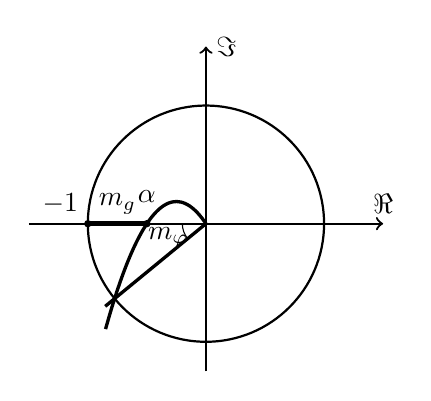
\begin{tikzpicture}[scale=1.5]
    \draw[->,thick](-1.5,0)--(1.5,0)node[above]{$\Re$};
    \draw[->,thick](0,-1.25)--(0,1.5)node[right]{$\Im$};

    \draw[thick](1,0)arc(0:360:1);
    \draw[very thick]plot[smooth, domain=-0.85:0](\x,{-3*\x*(\x+0.5)});

    \node[above left]at(-1,0){$-1$};
    \node[above]at(-0.5,0.1){$\alpha$};

    \draw[-, ultra thick](-1,0)--(-0.5,0);
    \filldraw[black](-1,0)circle(0.75pt);
    \filldraw[black](-0.5,0)circle(0.75pt);
    \node[above]at(-0.75,0){$m_g$};

    \coordinate(o)at(0,0);
    \coordinate(c)at(-0.773,-0.634);
    \coordinate(x)at(-0.5,0);
    \draw[very thick](0,0)--(-0.853,-0.7);
    \pic["$m_{\varphi}$", draw, angle eccentricity=1.7, angle radius=0.3cm]{angle=x--o--c};
\end{tikzpicture}
\end{document}